\documentclass[12pt,letterpaper]{article}
\usepackage{graphicx,textcomp}
\usepackage{natbib}
\usepackage{setspace}
\usepackage{fullpage}
\usepackage{color}
\usepackage[reqno]{amsmath}
\usepackage{amsthm}
\usepackage{fancyvrb}
\usepackage{amssymb,enumerate}
\usepackage[all]{xy}
\usepackage{endnotes}
\usepackage{lscape}
\newtheorem{com}{Comment}
\usepackage{float}
\usepackage{hyperref}
\newtheorem{lem} {Lemma}
\newtheorem{prop}{Proposition}
\newtheorem{thm}{Theorem}
\newtheorem{defn}{Definition}
\newtheorem{cor}{Corollary}
\newtheorem{obs}{Observation}
\usepackage[compact]{titlesec}
\usepackage{dcolumn}
\usepackage{tikz}
\usetikzlibrary{arrows}
\usepackage{multirow}
\usepackage{xcolor}
\newcolumntype{.}{D{.}{.}{-1}}
\newcolumntype{d}[1]{D{.}{.}{#1}}
\definecolor{light-gray}{gray}{0.65}
\usepackage{url}
\usepackage{listings}
\usepackage{color}
\usepackage{rotating}


\definecolor{codegreen}{rgb}{0,0.6,0}
\definecolor{codegray}{rgb}{0.5,0.5,0.5}
\definecolor{codepurple}{rgb}{0.58,0,0.82}
\definecolor{backcolour}{rgb}{0.95,0.95,0.92}

\lstdefinestyle{mystyle}{
	backgroundcolor=\color{backcolour},   
	commentstyle=\color{codegreen},
	keywordstyle=\color{magenta},
	numberstyle=\tiny\color{codegray},
	stringstyle=\color{codepurple},
	basicstyle=\footnotesize,
	breakatwhitespace=false,         
	breaklines=true,                 
	captionpos=b,                    
	keepspaces=true,                 
	numbers=left,                    
	numbersep=5pt,                  
	showspaces=false,                
	showstringspaces=false,
	showtabs=false,                  
	tabsize=2
}
\lstset{style=mystyle}
\newcommand{\Sref}[1]{Section~\ref{#1}}
\newtheorem{hyp}{Hypothesis}

\title{Problem Set 3}
\date{Due: March 24, 2024}
\author{Applied Stats II \\  Dan Zhang 23335541}


\begin{document}
	\maketitle
	\section*{Instructions}
	\begin{itemize}
	\item Please show your work! You may lose points by simply writing in the answer. If the problem requires you to execute commands in \texttt{R}, please include the code you used to get your answers. Please also include the \texttt{.R} file that contains your code. If you are not sure if work needs to be shown for a particular problem, please ask.
\item Your homework should be submitted electronically on GitHub in \texttt{.pdf} form.
\item This problem set is due before 23:59 on Sunday March 24, 2024. No late assignments will be accepted.
	\end{itemize}

	\vspace{.25cm}
\section*{Question 1}
\vspace{.25cm}
\noindent We are interested in how governments' management of public resources impacts economic prosperity. Our data come from \href{https://www.researchgate.net/profile/Adam_Przeworski/publication/240357392_Classifying_Political_Regimes/links/0deec532194849aefa000000/Classifying-Political-Regimes.pdf}{Alvarez, Cheibub, Limongi, and Przeworski (1996)} and is labelled \texttt{gdpChange.csv} on GitHub. The dataset covers 135 countries observed between 1950 or the year of independence or the first year forwhich data on economic growth are available ("entry year"), and 1990 or the last year for which data on economic growth are available ("exit year"). The unit of analysis is a particular country during a particular year, for a total $>$ 3,500 observations. 

\begin{itemize}
	\item
	Response variable: 
	\begin{itemize}
		\item \texttt{GDPWdiff}: Difference in GDP between year $t$ and $t-1$. Possible categories include: "positive", "negative", or "no change"
	\end{itemize}
	\item
	Explanatory variables: 
	\begin{itemize}
		\item
		\texttt{REG}: 1=Democracy; 0=Non-Democracy
		\item
		\texttt{OIL}: 1=if the average ratio of fuel exports to total exports in 1984-86 exceeded 50\%; 0= otherwise
	\end{itemize}
	
\end{itemize}
\newpage
\noindent Please answer the following questions:

\begin{enumerate}
	\item Construct and interpret an unordered multinomial logit with \texttt{GDPWdiff} as the output and "no change" as the reference category, including the estimated cutoff points and coefficients.\vspace{.15cm}\\
	\noindent First, let's load the data. Then, we need to convert \texttt{GDPWdiff} into factor. Next, run an unodered multinomial logit model with "no change" as the reference category.
	\lstinputlisting[language=R, firstline=40, lastline=52]{PS3.R}
	\noindent Here are the results:
	\begin{table}[!htbp] \centering   \caption{}   \label{} \begin{tabular}{@{\extracolsep{5pt}}lcc} \\[-1.8ex]\hline \hline \\[-1.8ex]  & \multicolumn{2}{c}{\textit{Dependent variable:}} \\ \cline{2-3} \\[-1.8ex] & negative & positive \\ \\[-1.8ex] & (1) & (2)\\ \hline \\[-1.8ex]  REG & 1.379$^{*}$ & 1.769$^{**}$ \\   & (0.769) & (0.767) \\   & & \\  OIL & 4.784 & 4.576 \\   & (6.885) & (6.885) \\   & & \\  Constant & 3.805$^{***}$ & 4.534$^{***}$ \\   & (0.271) & (0.269) \\   & & \\ \hline \\[-1.8ex] Akaike Inf. Crit. & 4,690.770 & 4,690.770 \\ \hline \hline \\[-1.8ex] \textit{Note:}  & \multicolumn{2}{r}{$^{*}$p$<$0.1; $^{**}$p$<$0.05; $^{***}$p$<$0.01} \\ \end{tabular} \end{table}
\newpage	
	\noindent Convert the coefficients into exponents:
		\lstinputlisting[language=R, firstline=53, lastline=54]{PS3.R}
	\begin{table}[!htbp] \centering   \caption{}   \label{} \begin{tabular}{@{\extracolsep{5pt}} cccc} \\[-1.8ex]\hline \hline \\[-1.8ex]  & (Intercept) & REG & OIL \\ \hline \\[-1.8ex] negative & $44.942$ & $3.972$ & $119.578$ \\ positive & $93.108$ & $5.865$ & $97.156$ \\ \hline \\[-1.8ex] \end{tabular} \end{table} 


	\noindent Interpretation:\\
	\texttt{Intercept: }
		\begin{itemize}
			\item "negative": The constant term of the "negative" category is 3.805, and the significance level is p$<$0.01, indicating that for a non-democracy country and its average ratio of fuel exports to total exports in 1984-86 no more than 50\%, the log odds of having a negative GDP difference versus no change is 3.805.

			\item "positive": The constant term of the "positive" category is 4.534 with a p$<$0.01, suggesting that for a non-democracy country and its average ratio of fuel exports to total exports in 1984-86 no more than 50\%, the odds of having a positive GDP difference  versus no change is 93.108.
		\end{itemize}
	
	\texttt{Coefficents of REG: }
		\begin{itemize}
			\item "negative": The coefficient is 1.379 with a p$<$0.1, indicating a statistically significant relationship at the 10\% level. This suggests that being a democracy (REG = 1) increases the log odds of having a negative GDP difference compared to no change by 1.379, when all other variables are held constant.
			
			\item "positive": The coefficient is 1.769 with a p$<$0.05, indicating a statistically significant relationship at the 5\% level. This implies that democracies have a positive GDP difference compared to no change, with the odds multiplying by a factor of 5.865 when all other variables are constant.
		\end{itemize}
		
	\texttt{Coefficients of OIL: }
		\begin{itemize}
			\item The coefficients for OIL are not statistically significant at the conventional levels (p$>$0.1). This suggests that the ratio of fuel exports to total exports does not significantly influence the likelihood of experiencing either a positive or negative GDP difference compared to no change.
		\end{itemize}
		
		
	\item Construct and interpret an ordered multinomial logit with \texttt{GDPWdiff} as the outcome variable, including the estimated cutoff points and coefficients.\vspace{.15cm}\\
	\noindent  First, let's convert  \texttt{GDPWdiff} into an ordered variable. Then, fit an ordered multinomial logit model.
	\lstinputlisting[language=R, firstline=59, lastline=63]{PS3.R}
	\noindent Here are the results:
	\begin{table}[!htbp] \centering   \caption{}   \label{} \begin{tabular}{@{\extracolsep{5pt}}lc} \\[-1.8ex]\hline \hline \\[-1.8ex]  & \multicolumn{1}{c}{\textit{Dependent variable:}} \\ \cline{2-2} \\[-1.8ex] & GDPWdiff \\ \hline \\[-1.8ex]  REG & 0.398$^{***}$ \\   & (0.075) \\   & \\  OIL & $-$0.199$^{*}$ \\   & (0.116) \\   & \\ \hline \\[-1.8ex] Observations & 3,721 \\ \hline \hline \\[-1.8ex] \textit{Note:}  & \multicolumn{1}{r}{$^{*}$p$<$0.1; $^{**}$p$<$0.05; $^{***}$p$<$0.01} \\ \end{tabular} \end{table}
	

	\noindent Let's calculate a p value for the model:
		\lstinputlisting[language=R, firstline=65, lastline=68]{PS3.R}
	\begin{table}[!htbp] \centering   \caption{}   \label{} \begin{tabular}{@{\extracolsep{5pt}} cccccc} \\[-1.8ex]\hline \hline \\[-1.8ex]  & Value & Std. Error & t value & p value & p value.1 \\ \hline \\[-1.8ex] REG & $0.398$ & $0.075$ & $5.300$ & $0.00000$ & $0.00000$ \\ OIL & $$-$0.199$ & $0.116$ & $$-$1.717$ & $0.086$ & $0.086$ \\ negative\textbar no change & $$-$0.731$ & $0.048$ & $$-$15.360$ & $0$ & $0$ \\ no change\textbar positive & $$-$0.710$ & $0.048$ & $$-$14.955$ & $0$ & $0$ \\ \hline \\[-1.8ex] \end{tabular} \end{table} 
	
	\noindent Convert the coeffiecients into exponents and add CIs:
		\lstinputlisting[language=R, firstline=70, lastline=71]{PS3.R}
	\begin{table}[!htbp] \centering   \caption{}   \label{} \begin{tabular}{@{\extracolsep{5pt}} cccc} \\[-1.8ex]\hline \hline \\[-1.8ex]  & OR & 2.5 \% & 97.5 \% \\ \hline \\[-1.8ex] REG & $1.490$ & $1.286$ & $1.727$ \\ OIL & $0.820$ & $0.655$ & $1.031$ \\ \hline \\[-1.8ex] \end{tabular} \end{table} 
	
	\noindent Interpretation:\\
	Check Table 3, we can see the coefficients of explanatory varibles are statistically significant. Let's interpret them respectively.\vspace{.25cm}\\
	\texttt{Coefficents of REG: } The coefficient for REG is 0.398 with a p-value $<$ 0.01, indicating a statistically significant positive association between being a democracy and the ordered level of GDP change. A positive coefficient suggests that as a country changes from non-democracy to democracy, the log odds of being in a higher category of difference of GDP also increase. The odds ratio for REG suggests that being a democracy increases the odds of experiencing a positive GDP change by 49\% compared to a non-democracy, holding all else constant. The confidence interval (1.286 to 1.727) does not include 1, confirming the statistical significance of this finding.
	
	\texttt{Coefficients of OIL: } The coefficient for OIL is -0.199 with a p-value $<$ 0.1, suggesting a statistically significant but negative relationship at the 10\% level. This implies that countries where fuel exports exceed 50\% of total exports are less likely to experience higher levels of GDP change. The presence of significant oil exports decreases the log odds of moving to a more positive category of GDP change.  The odds ratio for OIL indicates that countries with significant oil exports have 18\% lower odds of moving to a more positive GDP change category compared to countries without significant oil exports. The confidence interval (0.655 to 1.031) is close to including 1, indicating that this result is less robust and should be interpreted with caution.
	
\end{enumerate}

\newpage
\section*{Question 2} 
\vspace{.25cm}

\noindent Consider the data set \texttt{MexicoMuniData.csv}, which includes municipal-level information from Mexico. The outcome of interest is the number of times the winning PAN presidential candidate in 2006 (\texttt{PAN.visits.06}) visited a district leading up to the 2009 federal elections, which is a count. Our main predictor of interest is whether the district was highly contested, or whether it was not (the PAN or their opponents have electoral security) in the previous federal elections during 2000 (\texttt{competitive.district}), which is binary (1=close/swing district, 0="safe seat"). We also include \texttt{marginality.06} (a measure of poverty) and \texttt{PAN.governor.06} (a dummy for whether the state has a PAN-affiliated governor) as additional control variables. 

\begin{enumerate}
	\item [(a)]
	Run a Poisson regression because the outcome is a count variable. Is there evidence that PAN presidential candidates visit swing districts more? Provide a test statistic and p-value.\vspace{.15cm}\\
	\noindent First, let's load the data:
			\lstinputlisting[language=R, firstline=80, lastline=80]{PS3.R}
			
	\noindent Having a look at the data dispersion.
				\lstinputlisting[language=R, firstline=86, lastline=90]{PS3.R}
	\begin{figure}[htbp]
		\centering
		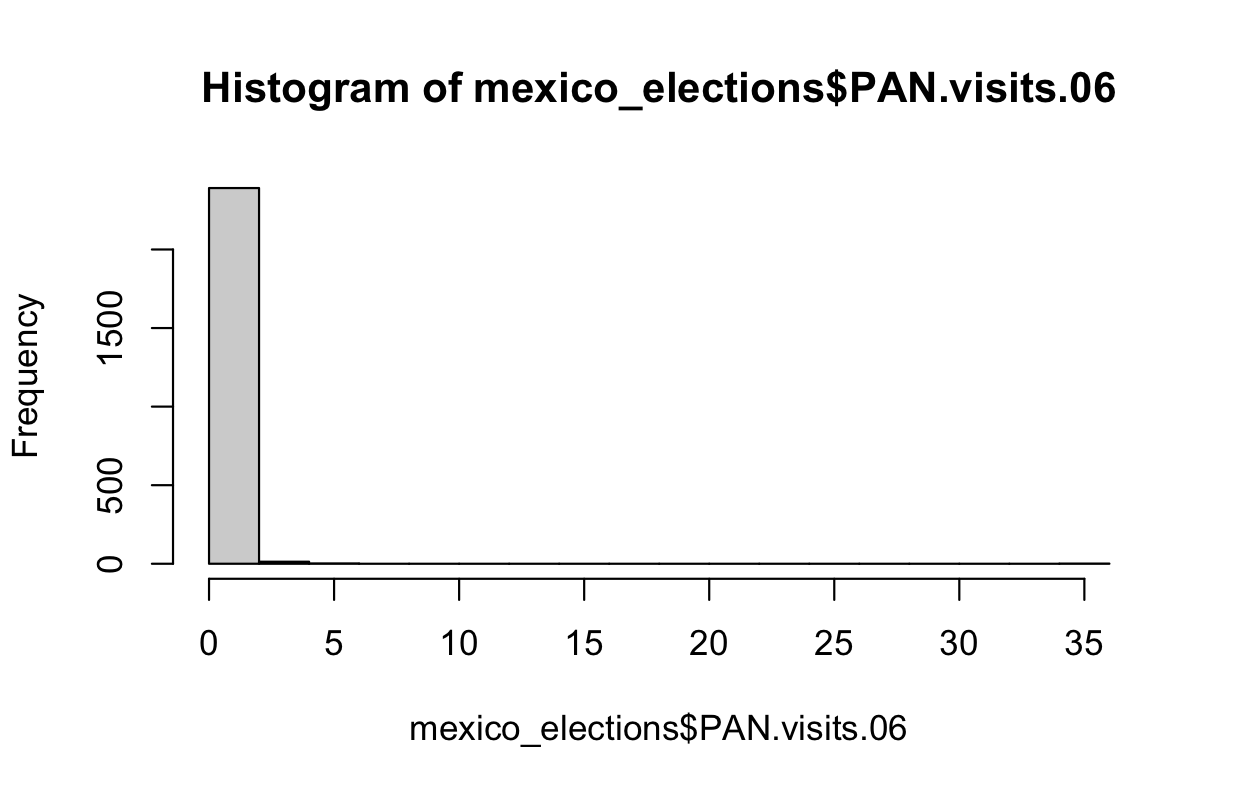
\includegraphics[width=0.8\textwidth]{Data dispersion histogram in R.png} 
		\caption{Outcome} 
		\label{fig: Outcome} 
	\end{figure}
	\begin{figure}[htbp]
		\centering
		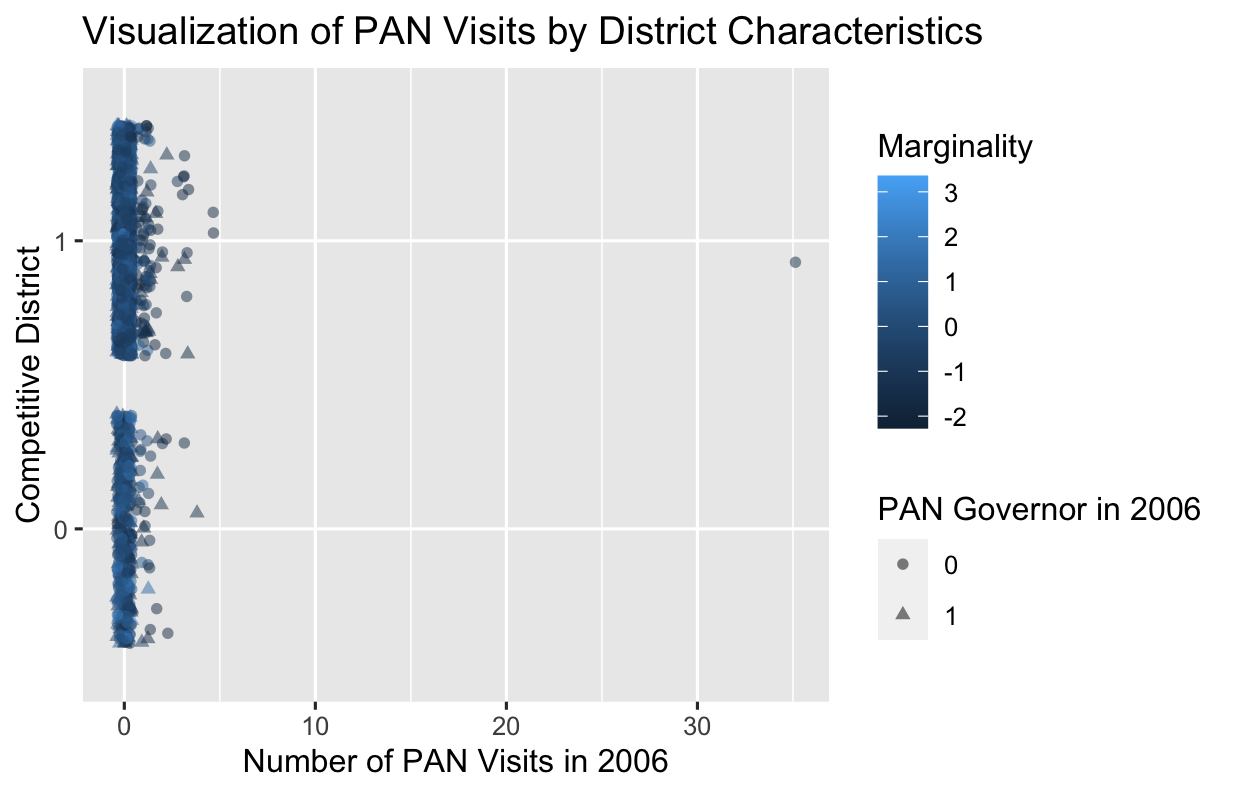
\includegraphics[width=0.8\textwidth]{Data dispersion in R.png} 
		\caption{Variables distribution} 
		\label{fig: Variables distribution} 
	\end{figure}
	
	\newpage
	\noindent By checking these pictures, we can see there are many zero values. In order to prevent over-dispersion problem, we need to run a dispersion test for poisson model. Let's run a poisson regression model.
			\lstinputlisting[language=R, firstline=93, lastline=94]{PS3.R}
	
	\noindent Run a dispersion test.
			\lstinputlisting[language=R, firstline=97, lastline=97]{PS3.R}
		\begin{table}[h]
			\centering
			\caption{Overdispersion Test Results}
			\begin{tabular}{l|l}
				\hline
				\textbf{Test Detail}            & \textbf{Result} \\
				\hline
				Data                            & model\_poisson \\
				Z-value                         & 1.0668 \\
				P-value                         & 0.143 \\
				Alternative Hypothesis          & True dispersion is greater than 1 \\
				Sample Estimates: Dispersion    & 2.09834 \\
				\hline
			\end{tabular}
			\label{tab:overdispersion}
		\end{table}
	
	\noindent As the p-value $=$ 0.143, the results are not statistically significant. There is not enough evidence to prove that there is an over-dispersion problem. Therefore, according to this test, he Poisson regression model is applicable for this dataset.

	\noindent Here are the test statistics and p values:
			\lstinputlisting[language=R, firstline=99, lastline=102]{PS3.R}
	\begin{table}[!htbp] \centering   \caption{}   \label{} \begin{tabular}{@{\extracolsep{5pt}} ccc} \\[-1.8ex]\hline \hline \\[-1.8ex]  & test\_statistic & p\_value \\ \hline \\[-1.8ex] (Intercept) & $$-$17.156$ & $0$ \\ competitive.district & $$-$0.477$ & $0.634$ \\ marginality.06 & $$-$17.728$ & $0$ \\ PAN.governor.06 & $$-$1.869$ & $0.062$ \\ \hline \\[-1.8ex] \end{tabular} \end{table}
	
	\noindent As we can see from the Table 6, the test-statistic coefficient for "competitive.district" is -0.477 with a p-value of 0.634. This suggests that, controlling all other variables constant in the model, being a competitive district does not have a statistically significant effect on the number of visits by PAN presidential candidates. The high p-value indicates that we fail to reject the null hypothesis of no effect. Besides, the coefficient of "competitive.district" is negative, which indicate that if this variable were statistically significant, it would indicate that competitive districts would have fewer PAN presidential candidate visits than non-competitive districts. However, due to the high p-value for this result, we cannot make this conclusion.

	\item [(b)]
	Interpret the \texttt{marginality.06} and \texttt{PAN.governor.06} coefficients.\vspace{.25cm}\\
	\noindent Here are the coefficients of the model:
	\begin{table}[!htbp] \centering   \caption{}   \label{} \begin{tabular}{@{\extracolsep{5pt}}lc} \\[-1.8ex]\hline \hline \\[-1.8ex]  & \multicolumn{1}{c}{\textit{Dependent variable:}} \\ \cline{2-2} \\[-1.8ex] & PAN.visits.06 \\ \hline \\[-1.8ex]  competitive.district & $-$0.081 \\   & (0.171) \\   & \\  marginality.06 & $-$2.080$^{***}$ \\   & (0.117) \\   & \\  PAN.governor.06 & $-$0.312$^{*}$ \\   & (0.167) \\   & \\  Constant & $-$3.810$^{***}$ \\   & (0.222) \\   & \\ \hline \\[-1.8ex] Observations & 2,407 \\ Log Likelihood & $-$645.606 \\ Akaike Inf. Crit. & 1,299.213 \\ \hline \hline \\[-1.8ex] \textit{Note:}  & \multicolumn{1}{r}{$^{*}$p$<$0.1; $^{**}$p$<$0.05; $^{***}$p$<$0.01} \\ \end{tabular} \end{table} 
	
	\begin{itemize}
		\item  \texttt{marginality.06}: The coefficient of \texttt{marginality.06} is -2.08 which is significantly negative (p $<$ 0.01). This indicates that as marginality (a measure of poverty) increases, the number of visits by PAN presidential candidates in 2006 decreases. Specifically, for a one-unit increase in marginality, the expected log count of PAN visits decreases by 2.080. This may suggest that PAN candidates were less likely to visit municipalities with higher levels of poverty in 2006.
		
		\item \texttt{PAN.governor.06}: The coefficient of \texttt{PAN.governor.06} is -0.312 which is also negative and statistically significant at the p $<$ 0.1 level. This suggests that the presence of a PAN-affiliated governor in the state is associated with a decrease in the number of visits by PAN presidential candidates. For districts within states governed by PAN in 2006, the expected log count of visits from PAN presidential candidates decreases by 0.312. This might imply that PAN candidates probably allocated their campaign efforts away from states already governed by their party, maybe focus on regions where gaining or maintaining political support was deemed more critical
	\end{itemize}
	
	\item [(c)]
	Provide the estimated mean number of visits from the winning PAN presidential candidate for a hypothetical district that was competitive (\texttt{competitive.district}=1), had an average poverty level (\texttt{marginality.06} = 0), and a PAN governor (\texttt{PAN.governor.06}=1).\vspace{.25cm}\\
	\noindent Use the predict function to check.
		\lstinputlisting[language=R, firstline=108, lastline=112]{PS3.R}
	\noindent The estimated mean number of visits would be 1.015 and its exponent value is 0.015. This means that the estimated mean number for a winning PAN presidential candidate to visit a competitive district which had an average poverty level and a PAN-affiliated governor is 1.015.
	
\end{enumerate}

\end{document}
